\documentclass[a4paper, 11pt]{article}

\usepackage{amsmath}
\usepackage{amssymb}
\usepackage{amsthm}
\usepackage{url}
\usepackage{graphicx}
\usepackage{hyperref}

% Theorem Styles
\newtheorem{theorem}{Theorem}[section]
\newtheorem{lemma}[theorem]{Lemma}
\newtheorem{proposition}[theorem]{Proposition}
\newtheorem{corollary}[theorem]{Corollary}
% Definition Styles
\theoremstyle{definition}
\newtheorem{definition}{Definition}[section]
\newtheorem{example}{Example}[section]
\theoremstyle{remark}
\newtheorem{remark}{Remark}

\begin{document}

\title{A predictive model for the Crowds protocol}
\date{\today}
\author{Marco Tinacci}
\maketitle

\section{Introduction}

\section{Preliminaries}
% TODO crowds protocol
% TODO dtmc
% TODO reachability probability

\section{Models}

\subsection{Input control array} \label{subs:inputcontrol}

\paragraph{Probabilistic behavior}
We model the protocol as a DTMC, states represent nodes of the network and edges represent transitions of the message from a node to another. Message forwarding is a probabilistic choice among nodes of the network. We can describe the dynamics of the protocol by using a stochastic matrix $A \in \mathbb{R}^{n\times n}$, with $n$ the number of nodes of the network. Since $A$ is stochastic the following condition holds

\begin{equation} \label{eq:stoc1}
a_{ij} \in [0,1],\ \forall i,j = 1,\dots,n
\end{equation}
\begin{equation} \label{eq:stoc2}
\sum_{i=1}^n a_{ij} = 1,\ \forall j = 1,\dots,n
\end{equation}

Let $a_{ij}$ be an element of $A$, we can describe how the dynamics modify the state using the following system

\begin{equation} \label{eq:system}
	x_j(k+1) = \sum_{i=1}^n a_{ij} x_i(k), \ \forall j = 1,\dots,n
\end{equation}

where the state $x(k) \in \mathbb{R}^n$ with $k \geq 0$ represents a probability distribution over states, then it holds $\sum_{i=1}^n x_i(k) = 1$ and $x_i(k) \in [0,1]$ for any $i = 1,\dots,n$.

\paragraph{Predictive control} % (fold)
\label{par:predictive_control}
We introduce a vector of parameters $u(k) \in \mathbb{R}^n$ at time $k$ that affect the system dynamics in the following way

\begin{equation} \label{eq:mpc}
		x(k+1) = Ax(k) + Bu(k)
\end{equation}

% TODO correggere dimensione B
for $k \in \mathbb{N}_0$ and $B \in \mathbb{R}^{n\times n}$. $B$ is a constant real square matrix that describe how parameters affect the state evolution.

% paragraph predictive_control (end)

\paragraph{Constraints} % (fold)
\label{par:constraints}
To preserve the probability distribution structure of the state we must ensure that, given any correct $x(k)$, the respective evolution $x(k+1)$ is still correct, that is $x(k+1) \in [0,1]^n$ and $\sum_{i=1}^n x_i(k+1) = 1$. From the former condition we derive the following constraints

\begin{equation} \label{eq:constr1}
	-1 \leq -\sum_j^n a_{ij} x_j(k) \leq \sum_j^m b_{ij} u_j(k) \leq 1 - \sum_j^n a_{ij} x_j \leq 1
\end{equation}
while, from the latter, we can derive
\begin{equation} \label{eq:constr2}
	\sum_{i=1}^n\sum_{j=1}^m b_{ij} u_j(k) = 0
\end{equation}


% paragraph constraints (end)

\paragraph{Objective} % (fold)
\label{par:objective1}
We use the canonical performance index (\ref{eq:performanceindex1}) for quadratic programming and we customize values in $P,Q \in \mathbb{R}^{n\times n}$ and $R \in \mathbb{R}^{m\times m}$ matrices to suit our target.
\begin{equation} \label{eq:performanceindex1}
	J(x(0),U) = x(N)^T P x(N) + \sum_{k=0}^{N-1} x(k)^T R x(k) + u(k)^T Q u(k)
\end{equation}
We are interested in maximizing the probability of being in a healthy node, with a priority for the receiver, and in minimizing the probability of using a corrupted node. 
% paragraph objective (end)

\paragraph{Results} % (fold)
\label{par:results}

We developed a MATLAB script that implement the crowds scenario we defined in this section. We used YALMIP to formulate the problem, generalizing it on the dimension of the network, on the number of corrupted nodes, on the number of parameters employed, on the length of the horizon and on the forward probability. In Figure~\ref{fig:results1} the predicted state behavior is represented (above) with the respective control actions (below) over time. We can see that healthy nodes (in blue) will be reached with a higher probability with respect to corrupted nodes (in red). The receiver (in green) has the highest probability due to the relatively high forward probability $p_f$. If we increase the number of control inputs, that in this test is $3$, the blu lines tend to move away from the red lines, still remaining close to each other, while red lines tend to move close to zero.

\begin{figure}[htbp]
	\begin{center}
	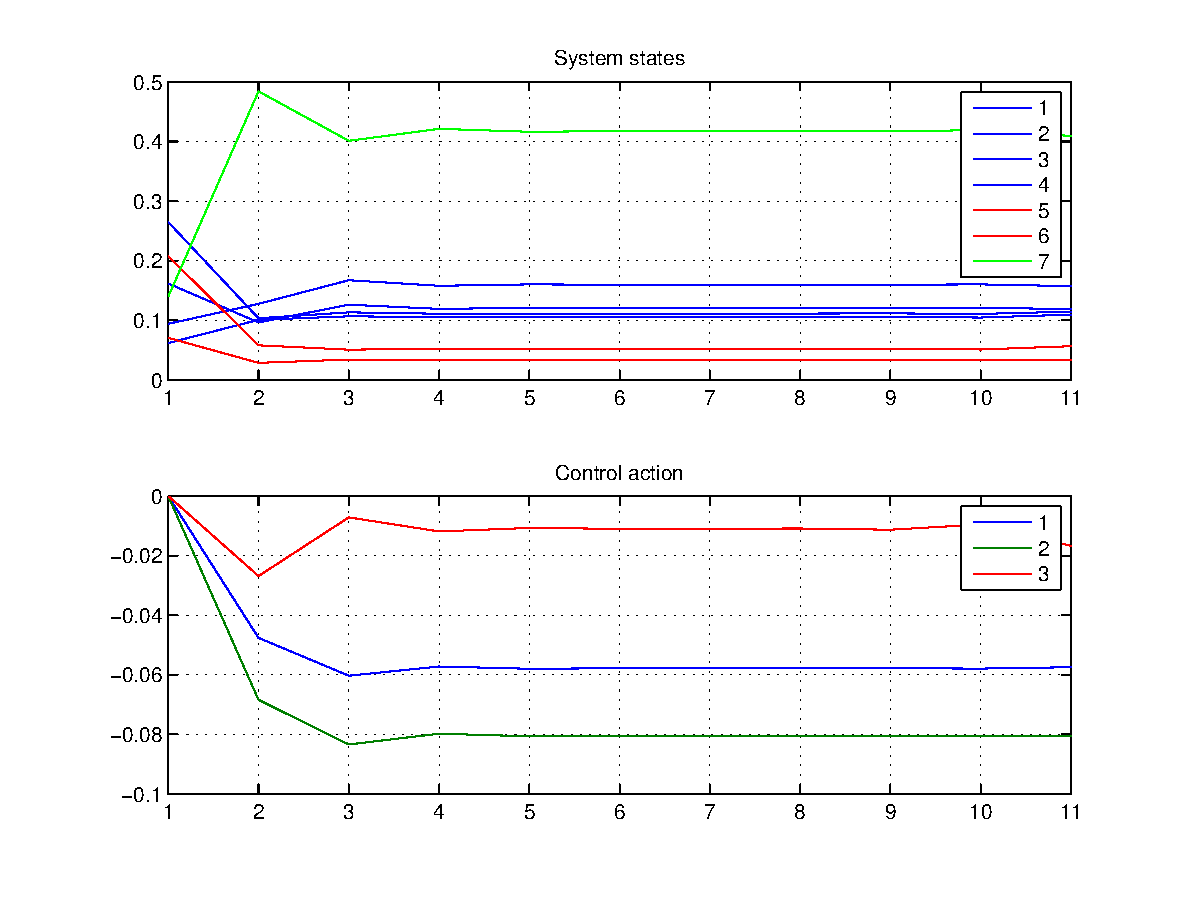
\includegraphics[width=.8\textwidth]{images/mpc}
	\end{center}
	\caption{Control of a crowds network of 7 nodes with 3 parameters with model predictive control}
	\label{fig:results1}
\end{figure}

The results represented in Figure~\ref{fig:results1} derive from an experiment with the following settings: 
\begin{itemize}
	\item the network contains $4$ healthy nodes, $2$ corrupted nodes and $1$ receiver;
	\item the prediction horizon is $10$;
	\item $3$ input parameters are used.
\end{itemize}
To maximize the probability of using a healthy node instead of a corrupted one we set weights in the performance index (\ref{eq:performanceindex1}) in the following way
\begin{equation} \label{eq:pqmatrix}
	P = Q = 10 \cdot I
\end{equation}
\begin{equation} \label{eq:rmatrix}
	r_{ij} = 
	\begin{cases}
		1 & \mbox{if } i=j \mbox{ and $i$ is a healthy node} \\
		10 & \mbox{if } i=j \mbox{ and $i$ is a corrupted node} \\
		0 & \mbox{if } i\neq j \\
	\end{cases}
\end{equation}
where $r_{ij}$ is an element of $R$. The MATLAB code used to run this experiment can be found in the github repository \url{https://github.com/marcotinacci/predictive-crowds/blob/master/mpc_crowds_yalmip.m}.
% paragraph results (end)

\subsection{Input control matrix}
We consider a variation of the control applied in the first model from Section~\ref{subs:inputcontrol}, since every input parameter may affect more than one transition probability and, on the other side, every probability could be affected by more than one input parameter. This kind of formulation does not make clear what control input actually are in the concrete scenario, thus we reformulate the problem in order to have a one-to-one relation between control inputs and transition probabilities. We consider the same stochastic matrix $A$ and constraints (\ref{eq:stoc1}) and (\ref{eq:stoc2}) to represent the system dynamics, but we change the control parameters in order to act on the specific transition probabilities.

\paragraph{Predictive control}
We introduce the possibility to tune probabilities over the edges of the Markov chain preserving the distribution constraints (\ref{eq:stoc1}) and (\ref{eq:stoc2}). Let $U \in \mathbb{R}^{n\times n}$ be the input matrix that will be used to tune the probabilities. In order to preserve the distribution constraints of $x(k)$ the following condition must hold on $U$
\begin{equation} \label{eq:zerosum}
	\sum_{j=1}^n u_{ij}(k) = 0
\end{equation}
where $u_{ij}(k)$ is an element of $U(k)$ and $k \geq 0$, for any $i = 1,\dots,n$.

Now we can extend the system dynamics (\ref{eq:system}) with parameters given by $U$ in this way
\begin{equation} \label{eq:system_extended}
	x_j(k+1) = \sum_{i=1}^n a_{ij} x_i(k) + u_{ij}(k), \ \forall j = 1,\dots,n
\end{equation}
It is easy to see that, if (\ref{eq:zerosum}) holds and $x(k)$ is a valid distribution, $x(k+1)$ is a distribution as well.

\paragraph{Constraints}
Since parameters $U(k)$ can increase or decrease transition probabilities $A$ out of the probability range $[0,1]$ we need to fix individual constraints to avoid that. Parameter $u_{ij}(k)$ is a local absolute modification of the probability mass flowing in a specific edge at time $k$, thus, starting from $a_{ij}x_j(k)+u_{ij}(k) \in [0,1]$ we can derive the following constraints

\begin{equation} \label{eq:constraints}
	-1 \leq -a_{ij}x_j(k) \leq u_{ij}(k) \leq 1-a_{ij}x_{j}(k) \leq 1
\end{equation}

\paragraph{Objective} % (fold)
\label{par:objective2}
We define a performance index with two features: firstly, minimizing the euclidean distance between the current state $x(k)$ and the ideal state $x_{id} \in [0,1]^n$, that is the distribution we want to obtain from the system; secondly, penalizing high modifications of input controls with specific costs. We use a weight vector $w^x$ to realize the former feature, while we use a weight matrix $W^u$ for the latter, to measure the effort of every input control on every probabilistic transition. The performance index is defined as follow
\begin{equation} \label{eq:index_ext}
	J(x(0),U) = \sum_{k=0}^{N-1}\sum_{i=1}^{n}\sum_{j=1}^{n} w_i^x(x_i(k) - x_{id})^2 + w_{ij}^u u^2_{ij}(k)
\end{equation}

Thus the problem can be summarize as the following optimization

\begin{equation} \label{eq:opt2}
	\begin{array}{ll}
		\underset{U}{\mbox{min}} & J(x(0),U) \\
		\mbox{subject to} &
		(\ref{eq:zerosum})(\ref{eq:system_extended})
		(\ref{eq:constraints}) \\
	\end{array}
\end{equation}


% paragraph objective (end)
\paragraph{Results} % (fold)
\label{par:results2}
Again we used the same environment (MATLAB + YALMIP) to formulate the problem and to solve it with quadratic programming. The result is shown in Figure~\ref{fig:results2} using the same notation from Figure~\ref{fig:results1}. The outcome is clearly more accurate than the previous experiment as expected, since we are using more parameters. To be specific we parametrize weights on edges instead of states. Moreover, we do not give a limit to the number of parameters that can be used.

Since the formulation of the problem is different, so it is the parameters setting. In this case we have to chose values for $w^x$, $w^u$ and $x_{id}$, while the rest of the values are the same as the previous experiment.

\begin{equation}
	\begin{array}{l}
		x_{id} = (0.05, 0.05, 0.05, 0.05, 0, 0, 0.8) \\
		w^x = (1, 1, 1, 1, 1, 1, 1) \\
		w^u = 
		\begin{pmatrix}
			0.1 & \cdots & 0.1 \\
			\vdots & \ddots & \vdots \\
			0.1 & \cdots & 0.1 \\
		\end{pmatrix} \\
	\end{array}
\end{equation}

\begin{figure}[htbp]
	\begin{center}
	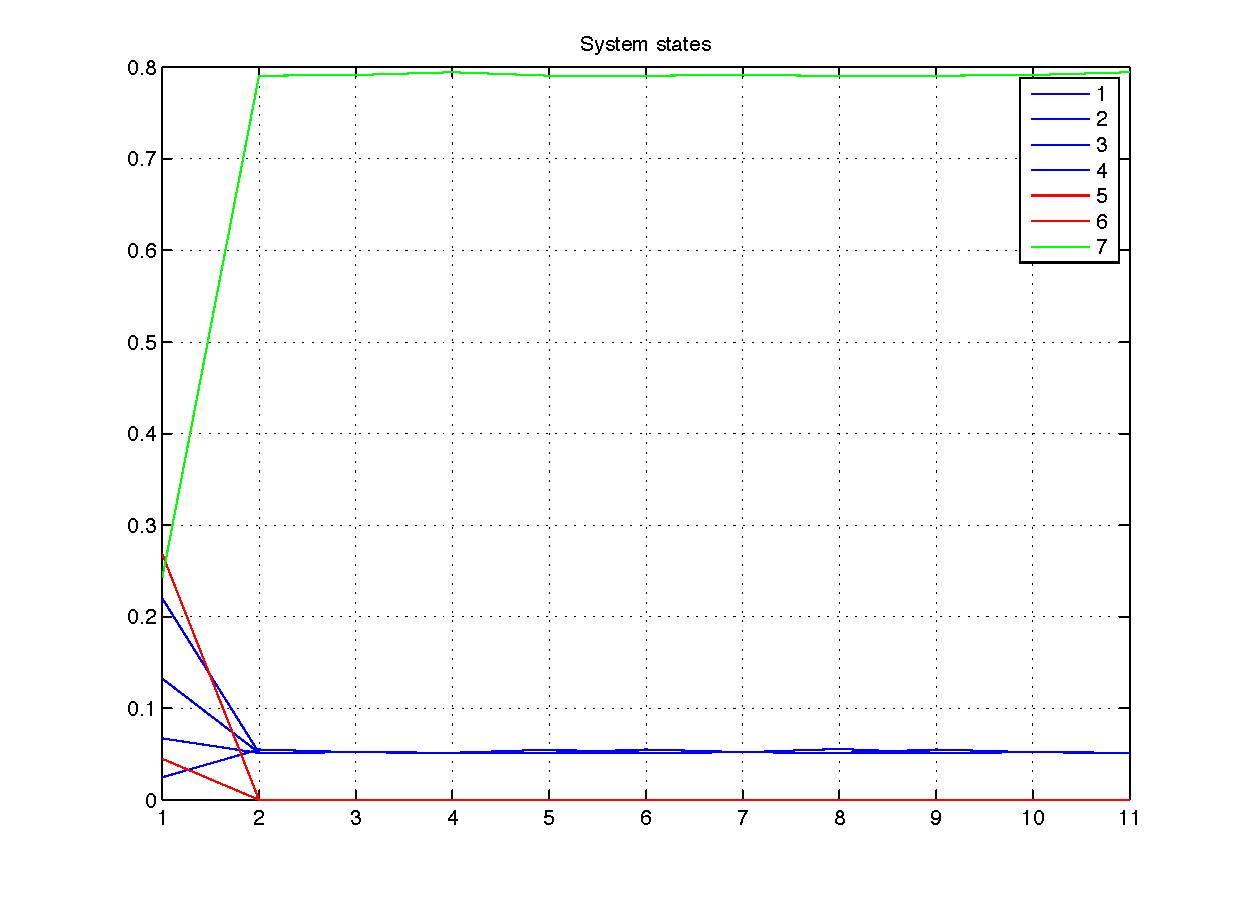
\includegraphics[width=.8\textwidth]{images/qp}
	\end{center}
	\caption{Control of a crowds network of 7 nodes with quadratic programming}
	\label{fig:results2}
\end{figure}




% paragraph results (end)
\section{Future work} % (fold)
\label{sec:future_work}

At the moment the scenario is not very realistic because we need to know which are the corrupted nodes before, but in that case any path avoiding those corrupted nodes would be a good solution. We could use the concept of partially observable model, like hidden Markov models, to model the perception of a leak of information. In this way penalties given to suspected corrupted nodes may be updated according to the perceived observations. Once the system has been modeled as a hidden Markov model, it can be converted into a discrete-time Markov chain and analyzed as we currently do. This kind of transformation is linear in the number of nodes times the number of observations.

In this work only the classical definition of the crowds protocol has been taken into account and the network is assumed to be strongly connected. Sparsity properties of different kind of topologies, block diagonal or band matrix structures for instance, may be exploited to improve analysis performance.
% section future_work (end)

\bibliographystyle{plain}
\bibliography{biblio}
% TODO paper crowd
% TODO yalmip
% TODO gurobi
% TODO repository github

\end{document}
